\documentclass[12pt]{article}
\usepackage{amssymb}
\usepackage{geometry}
\usepackage{graphicx}
\usepackage{hyperref}
\usepackage{wrapfig}
\usepackage{amsmath}
\usepackage{lipsum}
\usepackage{caption}
\usepackage{ulem}
\usepackage{xcolor}
\usepackage{tikz}
\usetikzlibrary{arrows.meta, positioning, shapes}

\usepackage{sectsty}
\sectionfont{\color{sectionColor}}       % Color for \section
\subsectionfont{\color{subsectionColor}}


\definecolor{titleColor}{HTML}{800000}        % Maroon
\definecolor{sectionColor}{HTML}{4682B4}      % SteelBlue
\definecolor{textHighlight}{HTML}{DAA520}     % Goldenrod
\definecolor{backgroundColor}{HTML}{F0F8FF}   % AliceBlue
\definecolor{emphasisColor}{HTML}{228B22}     % ForestGreen
\definecolor{subsectionColor}{HTML}{6A5ACD}   % SlateBlue


\title{\textcolor{titleColor}{\textbf{\Huge \textbf{Heart-hub a web application}}}}

\author{B. M. Osman\thanks{Al Nahada University, Cairo \\ \texttt{babikerosman@yahoo.com}}}
\date{\today}
\begin{document}
\maketitle



\begin{document}

The URL 
\url{https://hearthub-bjyb3bzoe-babikerosmans-projects.vercel.app/dashboard.html} 
points to a deployment of \textbf{HeartHub}, a web application hosted on Vercel.

HeartHub is an open-source Python toolkit by GitHub user 
\href{https://github.com/babikerosman468/Hearthub}{babikerosman468}, 
focusing on heart-based data science, coherent consciousness research, and community resilience modeling.

The GitHub repository provides backend tools and documentation, but does not include a detailed frontend dashboard.  The deployed URL appears to serve as a custom frontend interface.  Without access to the source code or further documentation, a detailed description of its functionalities is limited.
\begin{wrapfigure}{r}{0.35\textwidth}                       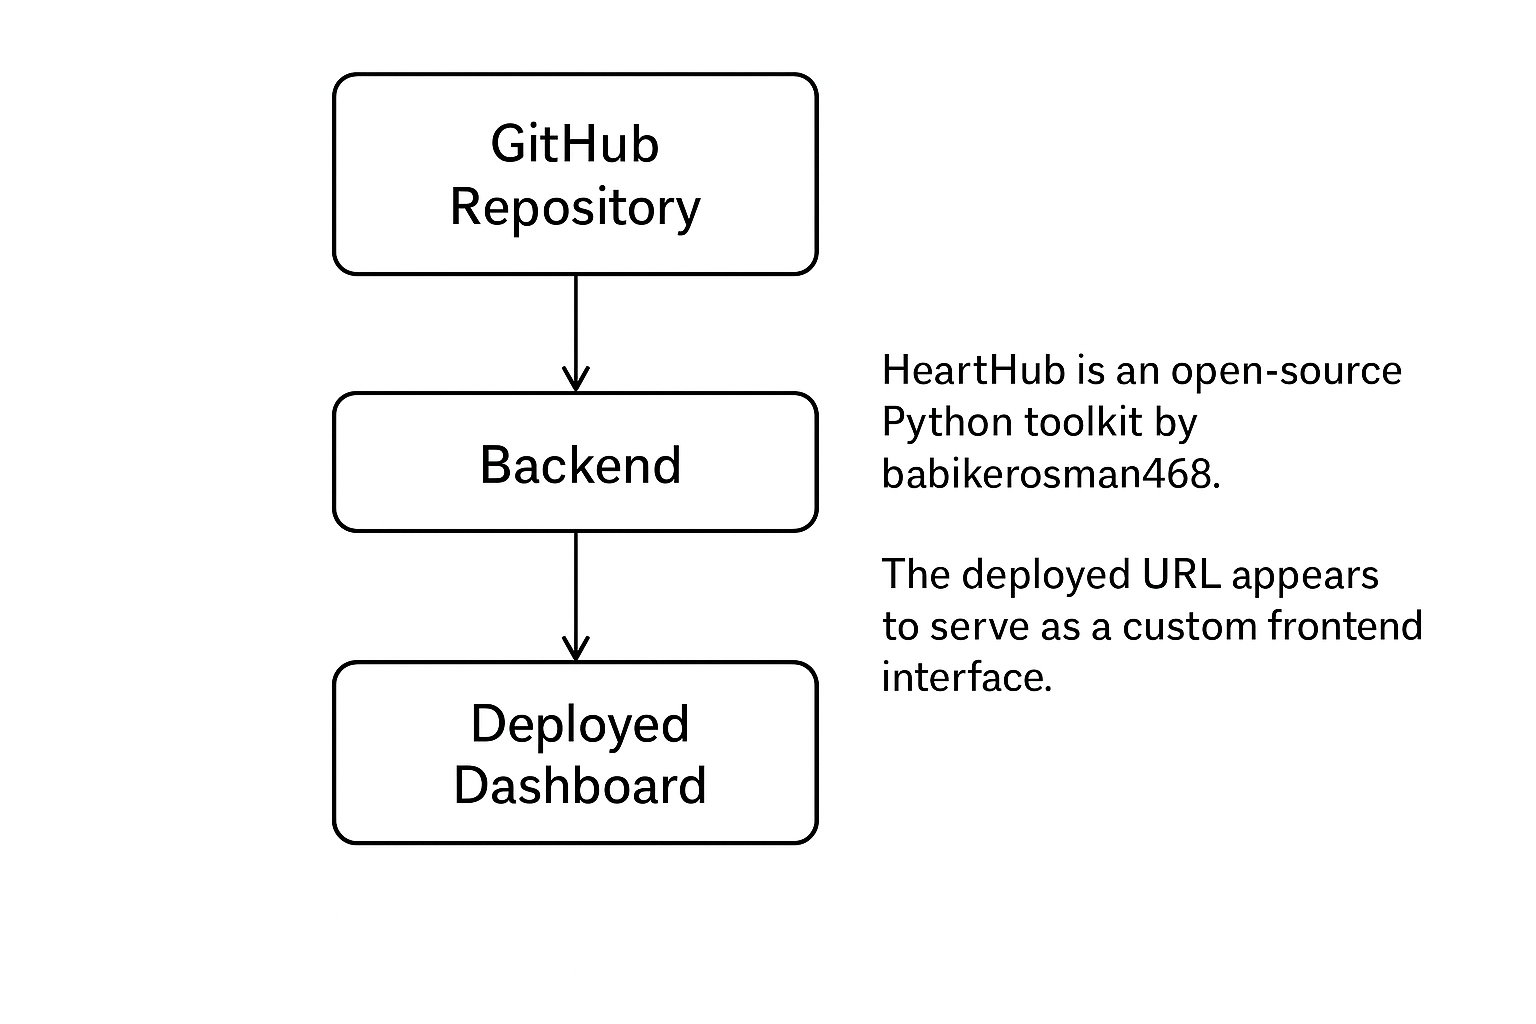
\includegraphics[width=0.35\textwidth]{6.png}
\caption{ \textbf{Hearthub} }      \end{wrapfigure}
For further exploration or contribution, the project repository can be accessed at 
\href{https://github.com/babikerosman468/Hearthub}{GitHub}.
\newpage


\par{\textcolor{titleColor}{\textbf{\Huge Hearthub Website: Public Deployment with Full Control}}}

% TikZ Styles
\tikzstyle{startstop} = [rectangle, rounded corners, minimum width=3.5cm, minimum height=1cm, text centered, draw=black, fill=red!30]
\tikzstyle{process} = [rectangle, minimum width=3.5cm, minimum height=1cm, text centered, draw=black, fill=blue!30]
\tikzstyle{decision} = [diamond, minimum width=3cm, minimum height=1cm, text centered, draw=black, fill=green!30]
\tikzstyle{arrow} = [thick,->,>=stealth]

\begin{center}
\begin{tikzpicture}[node distance=2cm]

% Nodes
\node (local) [process] {Edit Code Locally};
\node (git) [process, below of=local] {Push to Private Git Repository};
\node (deploy) [process, below of=git] {Deploy to Vercel (Public URL)};
\node (public) [startstop, below of=deploy] {Public Website};

\node (secret) [process, right of=git, xshift=6cm] {Environment Variables \& Secrets};
\node (admin) [process, right of=deploy, xshift=6cm] {Panel for Content Management};

% Arrows
\draw [arrow] (local) -- (git);
\draw [arrow] (git) -- (deploy);
\draw [arrow] (deploy) -- (public);

\draw [arrow] (git.east) -- (secret.west);
\draw [arrow] (deploy.east) -- (admin.west);

% Note
\node (note) [below of=public, yshift=-1.5cm, text width=12cm, align=center, color=emphasisColor] 
{\textit{Even though \textbf{Hearthub} is publicly accessible, full control can be maintained by managing the source code, deployment, and access carefully. 
The source code remains private, and sensitive information is secured. 
An optional \textbf{Admin Panel} allows content updates without exposing internal code. 
The workflow above illustrates the process.}};

\end{tikzpicture}
\end{center}

\end{document}
% Page setup
\geometry{a4paper, margin=1in}

